\documentclass{scrartcl}
\usepackage[ansinew]{inputenc}
%\usepackage[T1]{fontenc}
%\usepackage[ngerman]{babel} % Neue Rechtschreibung
\usepackage{amsmath} % Verbesserter Mathesatz
\usepackage{amssymb}
\usepackage{graphicx}
\usepackage[usenames,dvipsnames]{color}
\usepackage{listings}
\usepackage{hyperref}

\parskip1ex

\lstset{language=Java}
\lstset{numbers=right, numberstyle=\tiny, numbersep=5pt, tabsize=3, breaklines=true}
\lstset{basicstyle=\small\ttfamily,stringstyle=\ttfamily, keywordstyle=\color{blue}\bfseries,commentstyle=\color{OliveGreen}}

\begin{document}
\begin{titlepage}
\title{\begin{normalsize}Tutorial\end{normalsize} \\ Programming Tracker Software for ImageJ using the \texttt{PFTracking3D} Base Class}
\date{January 2008}
\author{Janick Cardinale \and \texttt{janickc@vision.ee.ethz.ch}}
\maketitle
\vspace{3cm}
\begin{center}
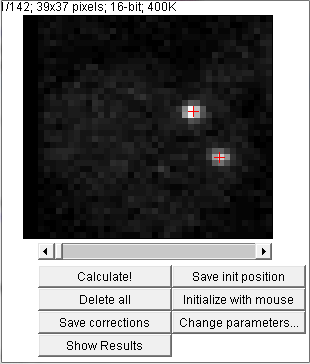
\includegraphics[width=.5\textwidth]{images/sampleTrack.png}
\end{center}
\thispagestyle{empty}
\newpage
\end{titlepage}
\setcounter{page}{1}

\tableofcontents

\section{Introduction}
\label{sec:introduction}
This tutorial shows how to use the PFTracking3D (PF stands for Particle Filtering) base class to implement a ImageJ tracking plugin and is further illustrated with an example that leads through the document. It is necessary to have some experience with the programming language Java. Some knowledge about particle filtering would be advantageously. 

The algorithm serves for tracking arbitrarily systems that can be described with a state vector and let you introduce easily the a-priori knowledge of the systems dynamics in 4D fluorescence microscopy. Prerequisites are that, first a state vector can uniquely describe your system and, secondly, that from such a state vector a resulting noise free expectation can be generated in an efficient way. Scruffy approximated images will introduce a bias. The algorithm is based on particle filtering. The more a-priori knowledge of the systems dynamics, the better will be the filtering and tracking results. If filtering of the systems dynamics is not desirable, the algorithm supports a local likelihood optimization (after applying the dynamics a-priori).

The data structures are prepared to track multiple objects in the same image. Note that there is no exclusion principle of different objects. If the a-priori knowledge is not sufficient, multi target tracking won't work (the trackers will collapse to the same object if the objects are too close to each other relative to their velocity).

\section{Preparation}
\subsection{Programming environment}
It is advisable to set up a Java programming environment like Eclipse\footnote{Eclipse - \href{http://www.eclipse.org}{http://www.eclipse.org}} or Netbeans\footnote{Netbeans - \href{http://www.netbeans.org}{http://www.netbeans.org}}. There are several possibilities to include ImageJs source code in the enviroenment, how to do that can be found at 'ImageJs Documentation Portal'\footnote{ImageJs Documentation Portal - \href{http://imagejdocu.tudor.lu/}{http://imagejdocu.tudor.lu/}}. Important is then that the base class and the derived class can be exported together in a \texttt{jar} archive. This archive can then be copied to ImageJs \texttt{Plugin} folder and after a restart of ImageJ, the plugin should start. These programming environments also enables you to profile your code and see where most of your calculation time was used. 

\subsection{Movies}
The base class was completely profiled and its architecture adapted such that optimal performance is achieved. Even though it is very recommendable to reduce the size of your movies as much as possible such that most of the image can be loaded in the CPUs cache memory. For example using the shortcut \texttt{Ctrl-D} in ImageJ crops a rectangular selection of your image. It does not matter if your movie is in 32 bit format, internally the image is converted to 32 bit anyway.

\section{An Example - Description of the System}
\label{sec:descriptionofthesystem}
The tutorial shows how to write a tracking plugin for a feature point with the constraint of inertia. The feature point is described by the coordinates, the velocities for each dimension and it's intensity. The acceleration of the feature point is modeled as Gaussian noise. The state vector is thus $\vec{x} = \left(x,y,z,v_x,v_y,v_z,I\right)$. 

\paragraph{Point Spread Function} The feature point convolved by the microscopes point spread function (PSF) is approximated by formula \ref{eq:idealimage}. The voxel $p = (p_x, p_y, p_z)^T$ has an intensity of:
\begin{equation}
\label{eq:idealimage}
	I(p_x,p_y,p_z|\vec{x}) = I \cdot \exp\left(\frac{-(x-p_x)^2}{2\sigma_{PSF_x}}-\frac{-(y-p_y)^2}{2\sigma_{PSF_y}}-\frac{-(z-p_z)^2}{2\sigma_{PSF_z}}\right)
\end{equation}

\paragraph{Dynamics} The dynamics model, describing the change of the state vector from frame $k$ to $k+1$, can be written in matrix form:
\begin{equation}
\label{eq:dynamicmodel}
\left[
\begin{array}{*{1}{c}}
	x_k \\
	y_k \\
	z_k	\\
	v_{x, k} \\
	v_{y, k} \\
	v_{z, k} \\	
	I_k
\end{array}
\right] = 
\left[
\begin{array}{*{7}{c}}
	1 & 0 & 0 & 1 & 0 & 0 & 0\\
	0 & 1 & 0 & 0 & 1 & 0 & 0\\
	0 & 0 & 1 & 0 & 0 & 1 & 0\\
	0 & 0 & 0 & 1 & 0 & 0 & 0\\
	0 & 0 & 0 & 0 & 1 & 0 & 0\\
	0 & 0 & 0 & 0 & 0 & 1 & 0\\
	0 & 0 & 0 & 0 & 0 & 0 & 1-\alpha\\
\end{array}
\right]\cdot
\left[
\begin{array}{*{1}{c}}
	x_{k-1} \\
	y_{k-1} \\
	z_{k-1}	\\
	v_{x, k-1} \\
	v_{y, k-1} \\
	v_{z, k-1} \\	
	I_{k-1}\\
\end{array}\right] + 
\left[
\begin{array}{*{1}{c}}
	0 \\
	0 \\
	0	\\
	a_x \\
	a_y \\
	a_z \\	
	a_I \\
\end{array}\right]
\end{equation}
with $\vec{a} \sim {\mathcal N}(0, Cov)$  and $a$ a random vector. $\alpha_k$ (may be progressive in time) describes the amount of bleaching of your fluorescent protein. The variances in vector $\vec{a}$ are determined by the user, see the method \texttt{showParamterDialog()} in section \ref{sec:methodsthatshouldbeoverrided}.

\paragraph{Background}
The background illumination is a parameter for the algorithm. But there is only support for a constant illumination. It is better to first subtract the local background. An appropriate plugin for ImageJ can be downloaded at CBLs homepage. Another is already implemented in ImageJ in the menu \texttt{Process->Subtract Background...}. It is not necessary to add a constant background to the image again; it is even better since the likelihood function, optimized by the algorithm in the base class, is more peaked and thus more precise (but with a too low signal strength (Intenstiy $<$ 11 photo-events), a non-neglectable bias is introduced). 

\section{Members and Data Structures}
\subsection{Important Member Variables}
\label{sec:importantmembervariables}
\paragraph{\texttt{mStateVectors}} The state vector of the actual calculated frame. The member is of type \lstinline[]{Vector<float[]>}. The float array is the actual state vector of an object. The vector holds references to all the objects to track. Important is, that there is a value assigned to the reference in the initialization procedure (\ref{sec:methodsthatshouldbeoverrided}).

\paragraph{\texttt{mStateVectorsMemory}} Holds references to all the state vectors of all the frames again in a \texttt{Vector} data type and is thus of type \lstinline[]{Vector<Vector<float[]>>}. Form this data structure, results can be read out, either to visualize them or to print them out. The size of the Vector is always as long as the movie is (number of frames). If there are no results at a certain frame, the vector holds \texttt{null} at this position. Please note that the index of the frames begins with 0. Generally framenumbers begin with index 1 (in the whole ImageJ application).

\paragraph{\texttt{mParticles}} Holds references to the current set of particles. To achieve this, the variables is chosen to be of type \lstinline[]{Vector<Vector<float[]>>}. The float array is a state vector with the weight/score of the particle appended at the last position of the array. For every object to track, several particles are necessary. This particles are stored as a \lstinline[]{Vector<float[]>} type. And for n objects, again a vector data type holds references to the objects particles vector.

\paragraph{\texttt{mParticlesMemory}} Holds information to all particles ever evaluated (for each frame) and is thus of type \lstinline[]{Vector<Vector<Vector<float[]>>>}. This information is only kept, if \texttt{mDoMonitorParticles} has the value 'true'. This may be useful to visualize the particles to investigate on the a-priori information and/or to debug.

\subsection{The Algorithms Parameters}
This section explains the meaning of all the parameters in the base class. All this parameters are implemented as member variables and have the prefix '\texttt{m}'.
\paragraph{\texttt{mNbOfThreads} - Number of Threads} The generation of the ideal image (see section \ref{sec:methodstooverride}) and the calculation of the likelihood function is invoked very frequently. Both operations are time consuming and are thus implemented such that they can be processed in parallel (for multicore CPUs). This parameter should comply with the number of cores of the computer.

\paragraph{\texttt{mNbOfParticles} - Number of Particles $\#p$} Specify how many particles are calculated per object, per frame and per optimization step. The calculation time of the algorithm is linear proportional to this parameter. On the other hand, a certain minimum of particles are required to achieve a good result.

\paragraph{\texttt{mRepSteps} - Number of Optimization Iterations} After applying the dynamic model, it may be useful to optimize the likelihood very locally. New particles are drawn and calculated gaussian distributed around the new estimated position of an object. The standard deviation of this Gaussian distribution is scaled down at every iteration according with factor $ s_k = \frac{1}{3^i}$ with $i = 1..mRepSteps$. If the algorithm detects, that there is not enough variation in the variance of the particles scores, it finishes to optimize even $i$ has not reached $mRepSteps$. 

\paragraph{\texttt{mResamplingThreshold} - Threshold $\theta$ for the Resampling Step} Normally only a few particles reach a high score. If so, all the particles are resampled (get all the same score and are moved to the position of the winning particles). This resampling step is triggered if \[
\theta > \frac{1}{\sum_{i=1}^{\#p}{w_i}^2}
\]
where $w_i$ is the weight (or score) of a certain particle.
\paragraph{\texttt{mBackground} - Constant Background Intensity} A constant background intensity added to the estimated images. This value has to be at least 1 (even if the background was subtracted by other software before).
\paragraph{\texttt{mSeed} - The Seed} Particle filtering is a stochastic optimization method. This variable is the seed used to construct the random generator. This seed should be also used in the derived class.
\paragraph{\texttt{mWaveLengthInNm} - Wave Length in Nanometer} The wave length of the light of the emitted by the fluorescent protein. 
\paragraph{\texttt{mNA} - Numerical Apparture} The Numerical Apparture (NA) of the microscope.
\paragraph{\texttt{mn} - The Refractive Index} The refractive index of the sample medium.
\paragraph{\texttt{mStateOfFilter} - State of the Plugin} This variable can take the following values: 
\begin{itemize}
	\item \texttt{WAITING = VISUALIZING = CORRECTING}: The plugin is doing nothing and waits either on a correct initialization or is showing it's results. If there is a frame with some data, the 'calculate' (from here) command is accepted.
	\item \texttt{INIT}: The state of the plugin has this value if the user clicked the 'initialize with mouse' button. The programmer may then interpret mouse events.
	\item \texttt{READY\_TO\_RUN}: The state after an initialization was done. The programmer may accept the 'calculate' command.
	\item \texttt{RUNNING}: While the algorithm is calculating.
\end{itemize}
\paragraph{\texttt{RESULT\_FILE\_SUFFIX}} The suffix for the generated result files. The files are written in the same directory as the movies are stored in. If the movie is not stored, the results are not stored neither but showed in a text window.
\paragraph{\texttt{INIT\_FILE\_SUFFIX}} The suffix for the generated initialization information files. The files contain all the information such that the plugin may start automatically (for batch processing with macros). The file is stored if the appropriate button was clicked by the user.

\section{Methods to Override}
\label{sec:methodstooverride}
In this section all the methods that have to be implemented by the programmer are presented and an example is given. The examples are related with the feature point tracker presented in section \ref{sec:descriptionofthesystem}. The full source code can be downloaded at the CBLs\footnote{CBL - Computational Biophysics Lab, Institute of Computational Science, Swiss Federal Institute of Technology (ETH), Zurich. \href{http://www.cbl.ethz.ch}{http://www.cbl.ethz.ch}} homepage. 

\subsection{Abstract Methods}
\label{sec:abstractmethods}
The first two methods presented in this chapter are the critical ones: The generation of an image given a certain state of the system and secondly, the implementation of the apriori knowledge of the dynamics. For this reason, this methods are presented in more detail here.

\paragraph{The Generation of an Expected Image} The method \texttt{generateIdealImage\_3D(...)} creates a 3D image in form of a three dimensional float array. The expected image to return represents how we expect the system to appear given a certain state vector. This state vector is passed as an argument \texttt{particle}. The dimensions of the image are also passed by arguments. 

Please note that this method is invoked very often and should be implemented as performant as possible. Generally, do not use setter and getter methods, they are to inefficient. Instead, use the arguments or member variables. Further, be sure that you only use thread safe data structures (or read only in this method). Do not change the particles content. 

In the following example, first the array to return is allocated. Afterwards, the background is added in a separate method that only adds the intensity to all the elements in the array. In line 4 the feature point intensities are added according to formula \ref{eq:idealimage}. 
\begin{lstlisting}
protected float[][][] generateIdealImage_3D(int aw, int ah, int as, float[] particle, int background, float pxWidthInNm, float pxDepthInNm) {

	float[][][] vIdealImage = new float[as][ah][aw];
	addBGToImage(vIdealImage, background);//not getMBackground()
	addFeaturePointTo3DImage(vIdealImage, ...);
	return vIdealImage;
}
\end{lstlisting}

\paragraph{Dynamics}
To introduce your prior knowledge of the systems dynamics, the programmer has to implement the method \texttt{drawFromProposalDistribution}. The argument array \texttt{aParticle} contains the old state of the particle and has to be updated here. The last entry of \texttt{aParticle} contains the particles weight, it is important to not change this entry. Except of the weight entry, a particle contains the same entry like the state vector. 
In the feature point example, entries 0 to 2 have to be updated by the velocities, this is done in line 3 (only for the x coordinate, the other coordinates are analogous). The velocity entries are updated by adding Gaussian noise (the acceleration). As a last thing, the intensity parameter is updated with a random walk model. With the last if condition it is guaranteed that the intensity never get smaller than the background. Note that this implementation corresponds to equation \ref{eq:dynamicmodel}: mSigma of dynamics correspond to the square root of the covariance matrix $Cov$ diagonal entry.
\begin{lstlisting}
protected void drawFromProposalDistribution(float[] aParticle, float aPxWidthInNm, float aPxDepthInNm) {
	particle[3] = particle[3] + mRandomGenerator.nextGaussian()*(mSigmaOfDynamics[0]/pxWidthInNm);
	particle[0] = particle[0] + particle[3];
	...
	/*repeat lines 2 and 3 for the y and z coordinate*/
	...
	//update the intensity value:
	particle[6] -= particle[6]*mAlpha;
	particle[6] += mRandomGenerator.nextGaussian()*mSigmaOfDynamics[3];
	//the intensity must not be smaller than the background:
	if(particle[6] < mBackground + 1)
		particle[6] = mBackground + 1;
}
\end{lstlisting}

\paragraph{Visualization} 
If you like to visualize the tracking results (very recommendable), for example to have a certain control if the algorithm breaked down while tracking, you can paint the results here on the canvas of the z-projected image using the \texttt{java.awt.Graphics} object passed by argument. The results can be taken from the mStateVectorsMemory member variable (see section \ref{sec:importantmembervariables}). The method \texttt{paintOnCanvas} may be returned immediately (without doing anything). 

In the feature point example it is first checked, if there really exist some data at the current frame by checking the vector element is equal to \texttt{null}. If not, the x and y coordinate (we paint on a z-projected frame) are read out from all the objects stored in the \texttt{mStateVectorsMemory} member variable. Afterward, a red cross is drawn on the \texttt{Graphics} object passed as an argument. The output can be seen on the titlepage of this document.
\begin{lstlisting}
protected void paintOnCanvas(Graphics aG, double magnification, int activeFrame) 
{
	if(mStateVectorsMemory.elementAt(activeFrame-1) == null)
		return;
	for(float[] vState:StateVectorsMemory.elementAt(activeFrame-1)){
		int vX = (int)Math.round(vState[0]*magnification+0.5f);
		int vY = (int)Math.round(vState[1]*magnification+0.5f);
		aG.setColor(Color.red);
		aG.drawLine(vX - 5, vY, vX + 5, vY); //draw a cross
		aG.drawLine(vX, vY - 5, vX, vY + 5);
	}
}
\end{lstlisting}

\paragraph{Getter Methods}
There are currently 3 getters necessary to implement:
\begin{itemize}
	\item A string that describe the dimensions of the state vector. This is then used to to print out in text windows or in files. In the feature point example, this is implemented as follows:
	\begin{lstlisting}
	public String[] getMDimensionsDescription() {
		String[] vS = {"x","y","z","vx","vy","vz","Intensity"};
		return vS;
	}
	\end{lstlisting}
	\item If you like to perform this optimization steps, return \texttt{true}, else return \texttt{false} in the \lstinline{public boolean getMDoPrecisionOptimization()}-method. Note that if you use this optimization procedure, you crucially reduce the filtering effect since the only the likelihood is optimized locally. In most of the cases this is favorable since we trust in the recorded images.
	\item To do the optimization steps, it is necessary to determine which parameter in the state vector should be optimized and how heavy they should be corrected. The float array to return contains the standard deviations of the first iteration of the likelihood optimization phase in the same order as the state vector stores the parameters. In the feature point example, only the coordinates (position 0,1 and 2) must be adapted (not the velocities!). Further we chose to also optimize the intensity dimension, thus position 7 in the array is set to 1:
	\begin{lstlisting}
	public float[] getMSigmaOfRandomWalk() {
		return new float[]{1f, 1f, 1f, 0, 0, 0, 1f};
	}	
	\end{lstlisting}
\end{itemize}

\subsection{Methods that should be overrided}
\label{sec:methodsthatshouldbeoverrided}
\begin{itemize}
\item{\lstinline{protected void mouseReleased(int ax, int ay)}} Mouse events invoke this methods, in this example it is a mouse release event. There are also methods to override for the mouse pressed, mouse clicked, mouse entered and mouse exited events. This methods are useful to design a mouse driven initialization procedure. 
How such an initialization may look like, you can see in the body of the feature point examples mouseReleased method:
\begin{lstlisting}
if(getMStateOfFilter() == STATE_OF_FILTER.INIT) {
	setMStateOfFilter(STATE_OF_FILTER.READY_TO_RUN);
	ImageStack vInitFrame = getAFrameCopy(getMOriginalImagePlus(), getMZProjectedImagePlus().getCurrentSlice());
	float[] vZInformation = calculateExpectedZPositionAt(ax, ay, vInitFrame);
	float[] vFirstState = new float[]{ax, ay, vZInformation[0], 0, 0, 0, vZInformation[1]};
	mStateVectors.add(vFirstState);
}
\end{lstlisting}
First, it is checked if the user first clicked the 'Initialize with mouse' button by checking the state of the filter. Afterwards the state is changed to 'ready to run' (see section \ref{sec:importantmembervariables}). Using the static method \texttt{getAFrameCopy} in the base class, the substack containing the activated frame in the projected image is copied to the \texttt{vInitFrame} variable. In line 4, the average of the brightest pixel on a ray through the stack at position \texttt{(ax,ay)} is calculated. In line 5 the state vector array of the feature point is created and finally added to the member \texttt{mStateVectors}.


\item{\lstinline{protected boolean[][][] generateParticlesIntensityBitmap_3D}} By implementing this method, the algorithm drastically speeds up its perfromance. The bitmap to return contains true if there is additianal (to the background) intensity at this position of the image added by any of the particle in this frame. So the programmer has three options. The first one is not to override the method. The base class implements this method by returning a bitmap that is true at all voxel. The second is to generate the bitmap while generating the ideal images (see method \texttt{generateIdealImage(...)}). The third is to iterate through all the particles like it is done in the feature point example. In each iteration, a bounding box by of the feature point is calculated. Within this bounding box, the bitmap is set to true. Of course, according to formula \ref{eq:idealimage}, each voxel is influenced by a feature point, but at a distance of $3\cdot \sigma_{PSF}$ the effect is neglected in the following method:

\begin{lstlisting}
protected boolean[][][] generateParticlesIntensityBitmap_3D(
			Vector<float[]> setOfParticles, int aW, int aH, int aS) {
	boolean[][][] vBitmap = new boolean[aS][aH][aW];
	//convert to pixel distance and multiply with 3:
	float vMaxDistancexy = 3*mSigmaPSFxy / getPixelWidthInNm();
	float vMaxDistancez = 3*mSigmaPSFz / getPixelDepthInNm(); 
	//get a bounding box around the each feature point
	int vXStart, vXEnd, vYStart, vYEnd, vZStart, vZEnd;
	for(float[] vParticle : setOfParticles) {
		if(vParticle[0] - vMaxDistancexy  < 0) 
			vXStart = 0; 
		else 
			vXStart = vParticle[0] - vMaxDistancexy;			
		if(vParticle[0] + vMaxDistancexy >= aW) 
			vXEnd = aW - 1; 
		else 
			vXEnd = vParticle[0] + vMaxDistancexy;
		...
		/*The same for the y and z dimension*/
		...
		for(int vZ = vZStart; vZ <= vZEnd; vZ++) 
			for(int vY = vYStart; vY <= vYEnd; vY++)
				for(int vX = vXStart; vX <= vXEnd; vX++)
					vBitmap[vZ][vY][vX] = true;								
	}
	return vBitmap;
}	
\end{lstlisting}

\item{\lstinline{protected boolean autoInitFilter(ImageStack aImageStack)}} If no initialization file is found at the movie files location, the programmer may try to initialize the first state vector automatically. If it is successful, return \texttt{true} in this method, else return \texttt{false}. The argument \texttt{aImageStack} is a frame to initialize and corresponds to the active frame before the plugin was started. The base class implementation simply returns \texttt{false}. In the feature point example, a little adapted k-means algorithm is used to initialize automatically. The calculation does not start automatically, even if the auto initailization was successful.

\item{\lstinline{protected void paintParticleOnCanvas(Graphics ag, float[] particle, double magnification)}} To debug or just to visualize where your particles are drawn, one may implement this method. With the member \texttt{mDoMonitorParticles} set to \texttt{true}, a separate black window with the same dimensions as your movie has, shows the particles. In the feature point example, just a small rectangle is drawn on the graphics object in the argument at the x and y position of the feature point, e.g. the first two elements in the \texttt{float[] particle} argument. The magnification argument contains the scalar that describe how much the window is scaled up by ImageJs magnification tool.

\item{\lstinline{protected boolean showParameterDialog()}}Before the calculation starts (after the 'calculate' butten was clicked), this method is invoked. Here the programmer may get the user defined parameters. It is important to use ImageJs \texttt{GenericDialog} class and its corresponding methods (like \texttt{addNumericField(...)} and \texttt{getNext-\hspace{0pt}
Number(...)}) such that macros will work. If the dialog was cancelled, the method should return \texttt{false}, else it should return \texttt{true}.

\end{itemize}

\section{Disclaimer}
IN NO EVENT SHALL THE ETH BE LIABLE TO ANY PARTY FOR DIRECT, INDIRECT, SPECIAL, INCIDENTAL, OR CONSEQUENTIAL DAMAGES, INCLUDING LOST PROFITS, ARISING OUT OF THE USE OF THIS SOFTWARE AND ITS DOCUMENTATION, EVEN IF THE ETH HAS BEEN ADVISED OF THE POSSIBILITY OF SUCH DAMAGE. THE ETH SPECIFICALLY DISCLAIMS ANY WARRANTIES, INCLUDING, BUT NOT LIMITED TO, THE IMPLIED WARRANTIES OF MERCHANTABILITY AND FITNESS FOR A PARTICULAR PURPOSE. THE SOFTWARE PROVIDED HEREUNDER IS ON AN "AS IS" BASIS, AND THE ETH HAS NO OBLIGATIONS TO PROVIDE MAINTENANCE, SUPPORT, UPDATES, ENHANCEMENTS, OR MODIFICATIONS.

%\section{Output Specification}

%\bibliographystyle{abbrv}
%\bibliography{refs}

\end{document}

